% (c) Jakub Stejskal
% Master Thesis
% Performance Testing and Analysis of Qpid-Dispatch Router
% Chapter 6

\chapter{Experimental Evaluation}
\label{Experimental Evaluation}
This chapter summarizes results of the performance testing and experimental evaluation with Maestro. We split the experiments into two parts. The first performs a basic measurement of Maestro\,1.3.0 which includes Maestro Agent and AMQP Inspector. During this measurements we focused on the highest possible throughput of singlepoint topology of Qpid-dispatch and Message Broker and multipoint topologies with three nodes of Qpid-dispatch and with Broker in the middle. The experimental topologies are depicted in the Figure \ref{fig:basic_topologies}. The later series of experiments focused on behavior testing of the topologies, which involves Qpid-Dispatch reliability and recovery testing.

Since the testing was executed over multiple topology types, we used Topology Generator for quick automatic changes of topology. Each test was executed against established topology where all components was newly installed and restarted between each test scenario. This was done during the cleaning stage. For experimental evaluation we used machines specified in the Table \ref{tab:machines}. The reason why the clients uses powerful machines is that we need more machines for SUT, but only two IBM Xeon machines was available during the experimental evaluation and we need at laest three machines for the SUT nodes.

% Please add the following required packages to your document preamble:
% \usepackage[table,xcdraw]{xcolor}
% If you use beamer only pass "xcolor=table" option, i.e. \documentclass[xcolor=table]{beamer}
\begin{table}[]
\centering
\caption{Machines and their properties, which were used for the experimental evaluation.}
\label{tab:machines}
\begin{tabular}{|l|l|r|r|}
\hline
\rowcolor[HTML]{C5E3DF}
\textbf{} & \multicolumn{1}{c|}{\cellcolor[HTML]{C5E3DF}\textbf{Machine}} & \multicolumn{1}{c|}{\cellcolor[HTML]{C5E3DF}\textbf{CPU}} & \multicolumn{1}{c|}{\cellcolor[HTML]{C5E3DF}\textbf{RAM (Gb)}} \\ \hline
SUT       & Opteron                                                       & 8                                                         & 8                                                      \\ \hline
Clients   & IBM Xeon                                                      & 16                                                        & 16                                                     \\ \hline
\end{tabular}
\end{table}

\section{Basic Performance Measurements}
\label{Basic Performance Measurements}
Maestro works as the orchestration system, and requires proper infrastructure before one can run any test for our experimental evaluation. The architecture of Maestro, described in the Chapter \ref{Messaging Performance Tool}, specifies that in ideal scenario one needs at least four machines for running a simple test: maestro broker, sender, receiver, and SUT. The amount of needed machines obviously rises with more complex scenarios and larger networks. Examples of generated experimental topologies are depicted in the Figures \ref{fig:basic_topologies}. For these configurations we compared the throughput and latency of these combination. During the all measurements we used Maestro Inspector for inspect one of the SUT depend on the topology type. Note, that for Qpid-Dispatch we used AMQP Inspector and for Broker we used Activemq Inspector. The topologies was picked based on current performance testing and known topologies, where was already found some performance degradation during the previous testing.

\begin{figure}[h]
	\centering
	\begin{minipage}{0.45\linewidth}
		\subfloat[Topology with a single router node.\label{fig:basic_topology_router}]{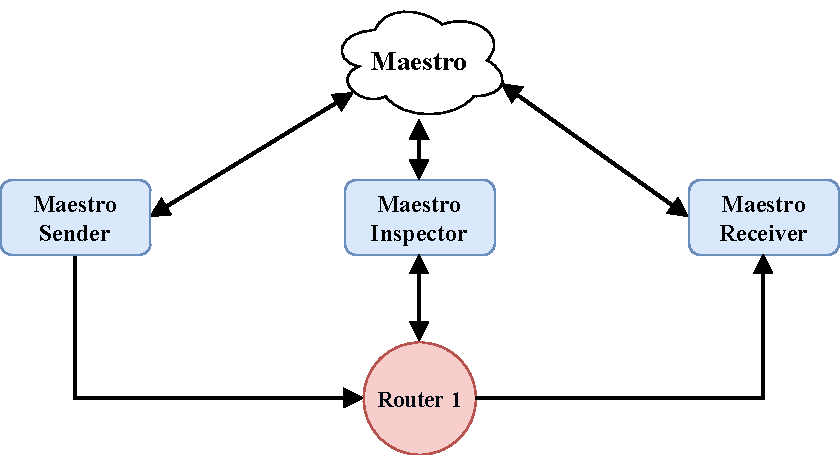
\includegraphics[width=\linewidth]{obrazky-figures/basic_topology_router_single.pdf}}
	\end{minipage}
	\begin{minipage}{0.45\linewidth}
		\subfloat[Topology with a single Broker node.\label{fig:basic_topology_broker}]{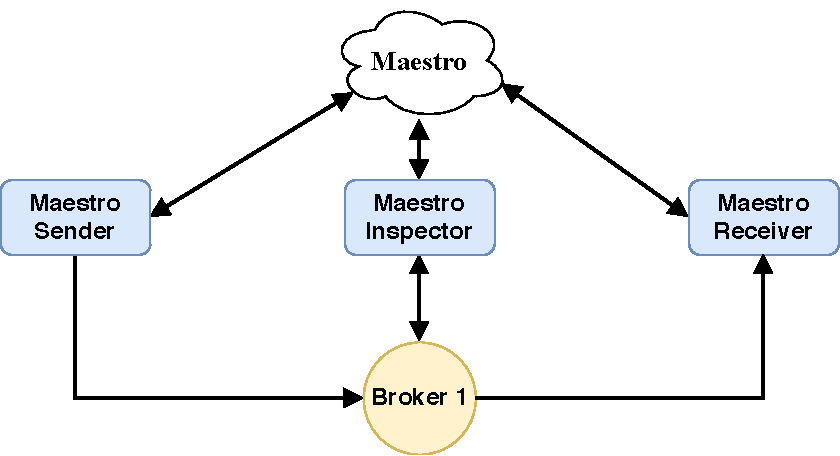
\includegraphics[width=\linewidth]{obrazky-figures/basic_topology_broker_single.pdf}}
	\end{minipage}
	\begin{minipage}{0.45\linewidth}
		\subfloat[Topology consisting of routers nodes only.\label{fig:basic_topology_router_line}]{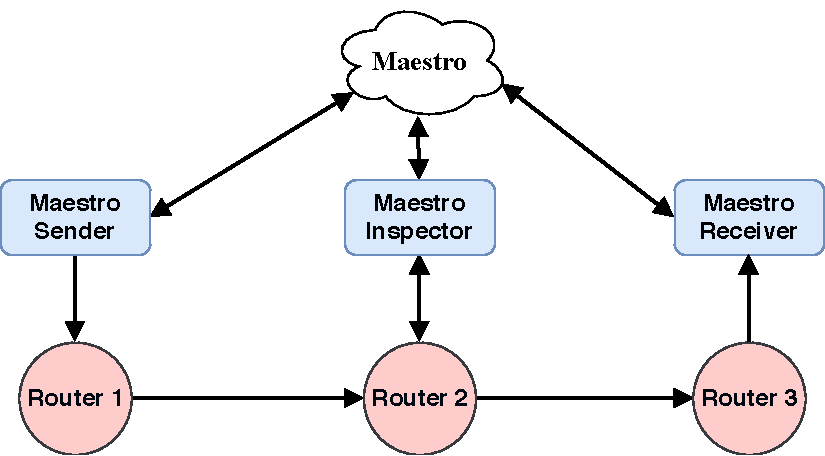
\includegraphics[width=\linewidth]{obrazky-figures/basic_topology_router.pdf}}
	\end{minipage}
	\begin{minipage}{0.45\linewidth}
		\subfloat[Topology with Broker in the middle.\label{fig:basic_topology_broker_line}]{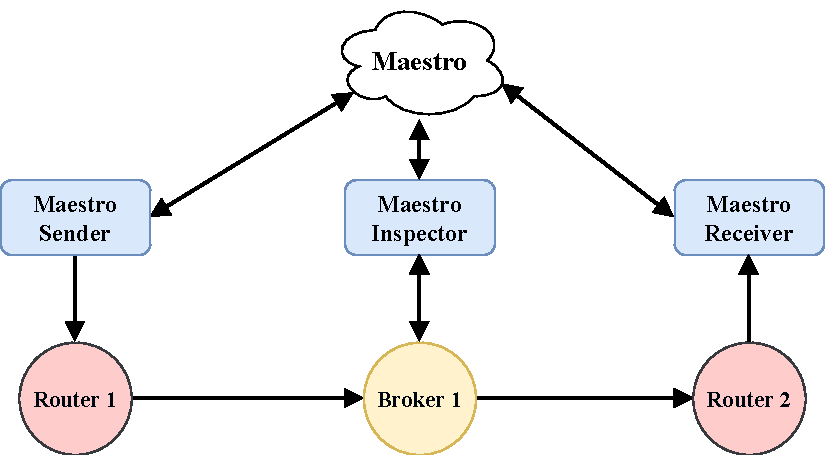
\includegraphics[width=\linewidth]{obrazky-figures/basic_topology_broker.pdf}}
	\end{minipage}
	\caption[Examples of experimental topologies created for basic performance testing and experiments with Maestro.]{Examples of experimental topologies created for basic performance testing and experiments with Maestro. The arrows indicates the communication path between the topology components.}\label{fig:basic_topologies}
\end{figure}

\subsection{Throughput}
\label{Throughput}
We measured throughput only by a load generators\,---\,\emph{Maes\-tro Sender} and \emph{Maestro Receiver}. Load generation depends on the test properties. One can see the test properties for each test case in the Table \ref{tab:test_case_throughput}. Maestro is able to create an unbounded rate test, during which it generates as much load as it can. This type of test was used to reach the maximum handled rate of Qpid-dispatch and Message Broker. The unbound rate during the test is achieved by set environment variable \emph{RATE} to value 0. The throughput test cases are focused on maximum throughput of simple or complex topology.

% Please add the following required packages to your document preamble:
% \usepackage{multirow}
% \usepackage[table,xcdraw]{xcolor}
% If you use beamer only pass "xcolor=table" option, i.e. \documentclass[xcolor=table]{beamer}
\begingroup
\setlength{\tabcolsep}{10pt} % Default value: 6pt
\renewcommand{\arraystretch}{1.35} % Default value: 1
	\begin{table}[H]
	\centering
	\caption{Test case settings for throughput measurements}
	\label{tab:test_case_throughput}
	\begin{tabular}{|l|r|r|r|r|}
	\hline
	\rowcolor[HTML]{C5E3DF}
	\cellcolor[HTML]{C5E3DF}                                         & \multicolumn{4}{c|}{\cellcolor[HTML]{C5E3DF}\textbf{Value}}                                                                          \\ \cline{2-5}
	\rowcolor[HTML]{C5E3DF}
	\cellcolor[HTML]{C5E3DF}                                         & \multicolumn{2}{c|}{\cellcolor[HTML]{C5E3DF}\textbf{Singlepoint}} & \multicolumn{2}{c|}{\cellcolor[HTML]{C5E3DF}\textbf{Multipoint}} \\ \cline{2-5}
	\rowcolor[HTML]{C5E3DF}
	\multirow{-3}{*}{\cellcolor[HTML]{C5E3DF}\textbf{Test Property}} & \textbf{Router}                 & \textbf{Broker}                 & \textbf{Full Router}            & \textbf{With Broker}           \\ \hline
	\textbf{MESSAGE\_SIZE}                                           & \multicolumn{4}{c|}{256}                                                                                                             \\ \hline
	\textbf{PARALLEL\_COUNT}                                         & \multicolumn{4}{c|}{5}                                                                                                               \\ \hline
	\textbf{TEST\_DURATION}                                          & \multicolumn{4}{c|}{15m}                                                                                                             \\ \hline
	\textbf{RATE}                                                    & \multicolumn{4}{c|}{\cellcolor[HTML]{FFFFFF}0}                                                                                       \\ \hline
	\end{tabular}
	\end{table}
\endgroup

\subsubsection*{Single Node}
The first of tests were ran against the single node topologies, which are depicted in the Figures \ref{fig:basic_topology_router} and \ref{fig:basic_topology_broker}. These topologies contains only one SUT node, which are forwarding messages from sender to receiver. During the test is the SUT node inspected by the proper Maestro Inspector.

The measured throughput is depicted in the Figure \ref{fig:rate-single} where one can see the comparison of tests with 15\,minutes duration, which is oriented to achieve highest possible throughput. The one can see that maximum throughput of Qpid-Dispatch as an standalone network component can reach around 90\,0000 messages per second. On the other hand, the lone Messaging Broker reaches only about 30\,000 messages per second. This throughput difference is caused by the fact, that Broker stores all of the messages in the memory till the clients want them. This is main feature of the broker, cause it operates as an message distributor in the network. The router only routes the messages to the destination which does not need to store message in the memory.

\begin{figure}[H]
	\centering
	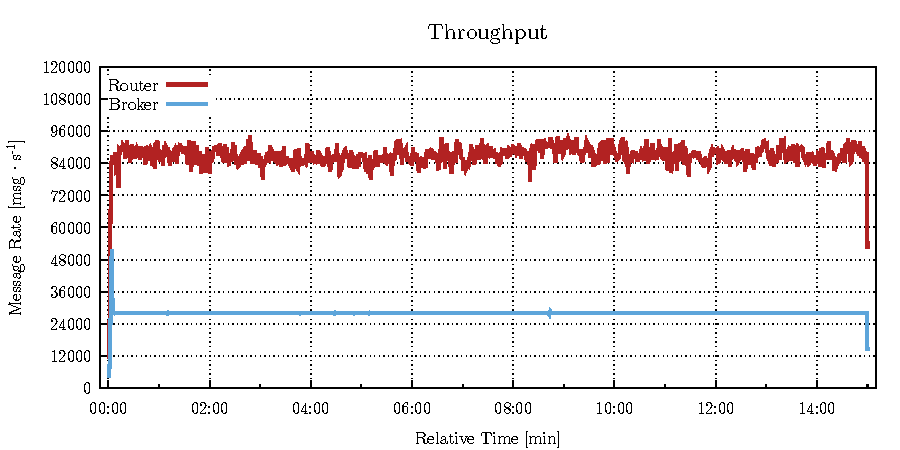
\includegraphics[width=1\linewidth]{obrazky-figures/charts/singlepoint-throughput.pdf}
	\caption{Chart of the maximum throughput of router and broker during the singlepoint test case. One can see here the difference between those two components.}
	\label{fig:rate-single}
\end{figure}

In the Figure \ref{fig:router-single-memory} we can see the memory usage of Qpid-dispatch during the test. We can see here, that totally allocated is around 45\,KB from which is used around 13\,---\,28\,KB. If we compare this with the memory allocation for the Broker, we can see the huge difference between these values. The memory allocated for the Broker is depicted in the Figure \ref{fig:broker-single-memory}. Here we can see that allocated is around 2\,GB of memory and used is around 300\,---\,900\,MB. This is caused by the store message in the memory.

\begin{figure}[H]
	\centering
	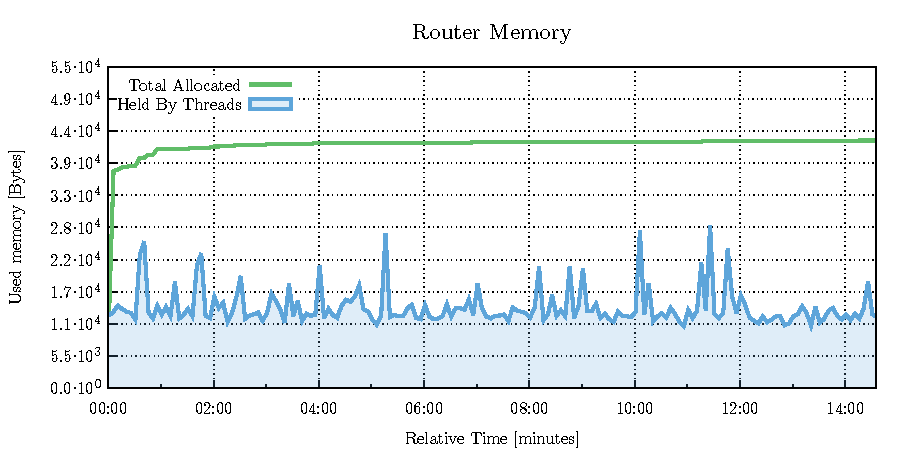
\includegraphics[width=1\linewidth]{obrazky-figures/charts/singlepoint-router-throughput-memory.pdf}
	\caption{The allocated memory and memory in use by Qpid-Dispatch during the test. The data was collected by the inspector every 5\,seconds.}
	\label{fig:router-single-memory}
\end{figure}

\begin{figure}[H]
	\centering
	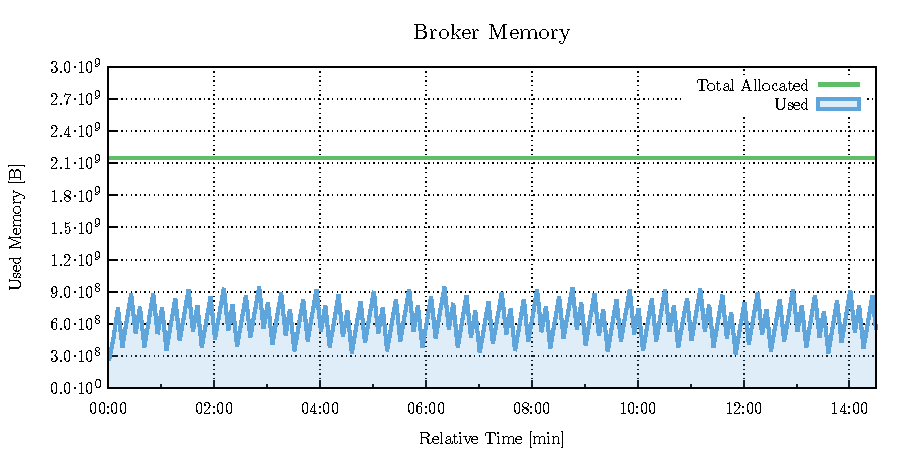
\includegraphics[width=1\linewidth]{obrazky-figures/charts/singlepoint-broker-throughput-memory.pdf}
	\caption{The memory allocation for the Broker service. One can see that the broker allocates more memory than Qpid-Dispatch.}
	\label{fig:broker-single-memory}
\end{figure}


\subsubsection*{Multipoint Topology}
For the multipoint experiments were used topologies depicted in the Figures \ref{fig:basic_topology_router_line} and \ref{fig:basic_topology_broker_line}. The network throughput can be influenced by another devices connected to the topology. The singlepoint topology was extended by another components by add two other routers around the original SUT. The versions of the new added SUTs are the same as the original ones.

\begin{figure}[H]
	\centering
	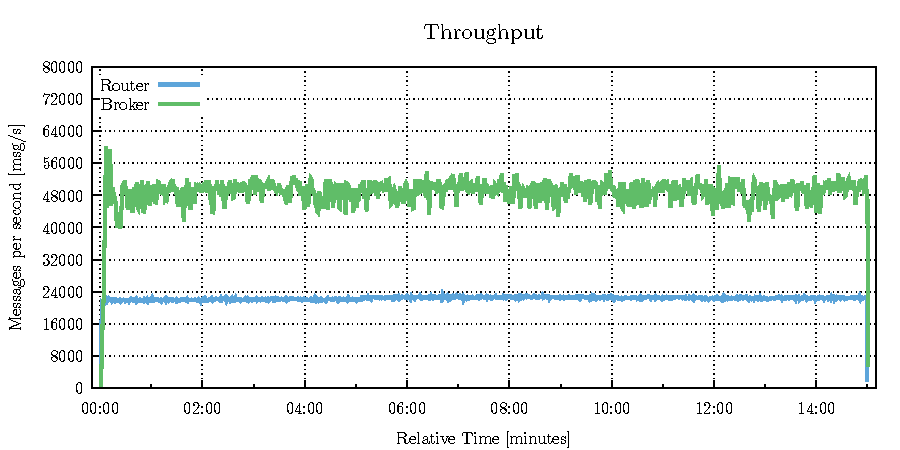
\includegraphics[width=1\linewidth]{obrazky-figures/charts/multipoint-throughput.pdf}
	\caption{Measured throughput of Qpid-Dispatch and Message Broker during the multipoint case study. One can see the performance degradation of Qpid-Dispatch and improvements of Message Broker on that Figure.}
	\label{fig:rate-multipoint-router}
\end{figure}

In the Figure \ref{fig:rate-multipoint-router} one can see, that the adding the routers to the broker node raises achievable throughput to the 48\,000 messages per second. However, the topology consists only of the routers has significant performance degradation. The throughput falls from the 90\,000 messages per second to the approximately 23\,000 messages per second. This degradation is caused by the interior flow-control mechanism, which should prevent the overload of the network. However, in this case study we can see that the performance degradation is too high and the mechanism used in the Qpid-Dispatch should be re-implemented.


\begin{figure}[H]
	\centering
	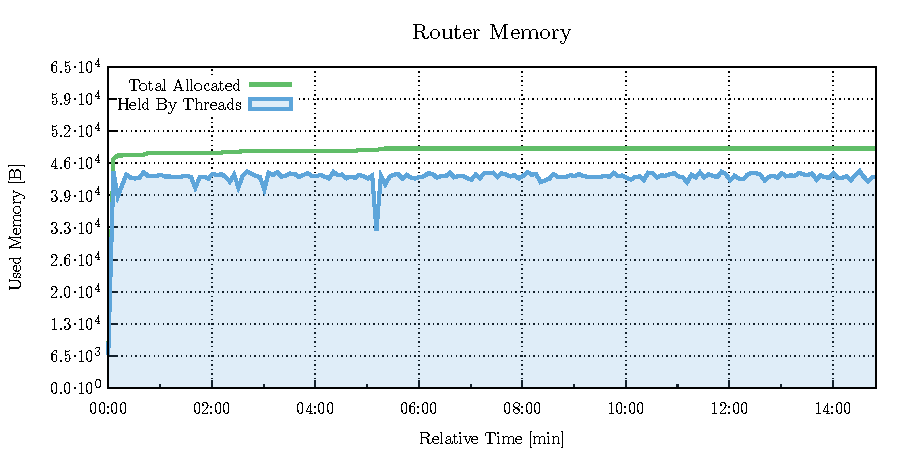
\includegraphics[width=1\linewidth]{obrazky-figures/charts/multipoint-router-only-throughput-memory.pdf}
	\caption{Qpid-Dispatch's memory usage during the multipoint case study. Used memory is higher than in previous case.}
	\label{fig:router-multipoint-memory}
\end{figure}

Based on that mechanism, the memory usage of the middle router depicted in the Figure \ref{fig:router-multipoint-memory} is higher than during the previous case study. Memory used by all threads is there sometimes two times higher and the mean value is around 43\,KB. On the other the, memory allocated for the broker component remains the same as in the previous case study. The memory monitoring for this case study is depicted in the Figure \ref{fig:broker-multipoint-memory}.

\begin{figure}[H]
	\centering
	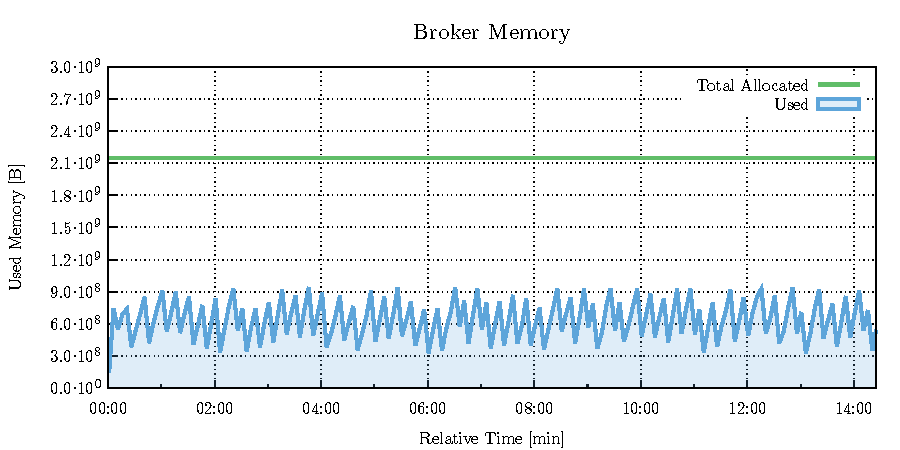
\includegraphics[width=1\linewidth]{obrazky-figures/charts/multipoint-router-broker-throughput-memory.pdf}
	\caption{Memory usage for Broker remains almost the same like in the previous case with less spikes.}
	\label{fig:broker-multipoint-memory}
\end{figure}


\subsubsection*{Conclusion}
The collected data during the throughput measurements reveals unexpected and considerable performance degradation in the serial connection of the Qpid-Dispatch. For comparison between the single and multipoint case study here is the Figure \ref{fig:basic-throughput-comparison}, which puts together all throughput measurements data into one chart. Here one can see the performance improvement between single instance Broker test and the test of topology with the broker (yellow and green color), and performance degradation between router topologies (red and blue color). The results are also available in the Table \ref{tab:throughput-summary}.

% Please add the following required packages to your document preamble:
% \usepackage{multirow}
% \usepackage[table,xcdraw]{xcolor}
% If you use beamer only pass "xcolor=table" option, i.e. \documentclass[xcolor=table]{beamer}
\begingroup
\setlength{\tabcolsep}{10pt} % Default value: 6pt
\renewcommand{\arraystretch}{1.35} % Default value: 1
	\begin{table}[h]
	\centering
	\caption{Table with collected data with highlighted performance improvements and degradations.}
	\label{tab:throughput-summary}
	\begin{tabular}{|l|r|r|r|r|}
	\hline
	\rowcolor[HTML]{C5E3DF}
	\cellcolor[HTML]{C5E3DF}                                         & \multicolumn{2}{c|}{\cellcolor[HTML]{C5E3DF}\textbf{Throughput (Msg/s)}}             & \multicolumn{2}{c|}{\cellcolor[HTML]{C5E3DF}\textbf{Memory}} \\ \cline{2-5}
	\rowcolor[HTML]{C5E3DF}
	\multirow{-2}{*}{\cellcolor[HTML]{C5E3DF}\textbf{Test Type}} & \textbf{Expected}             & \textbf{Measured}                                    & \textbf{Total}              & \textbf{Used max}              \\ \hline
	\textbf{Single Router}                                           & -                             & 90\,000                                                & 45\,MB                       & 28\,MB                          \\ \hline
	\textbf{Single Broker}                                           & -                             & 30\,000                                                & 2\,GB                        & 0.9\,GB                         \\ \hline
	\textbf{Line of Routers}                                         & 90\,000                         & \cellcolor[HTML]{FFCCC9}23\,000                        & 49\,MB                       & 43\,MB                          \\ \hline
	\textbf{Line with Broker}                                        & 30\,000 & \cellcolor[HTML]{9AFF99}48\,000 & 2\,GB                        & 0.9\,GB                         \\ \hline
	\end{tabular}
	\end{table}
\endgroup

\begin{figure}[H]
	\centering
	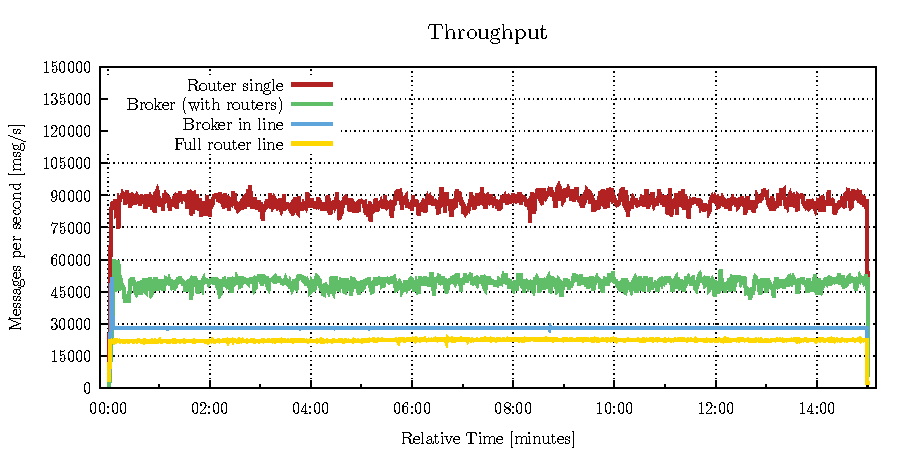
\includegraphics[width=1\linewidth]{obrazky-figures/charts/basic-throughput.pdf}
	\caption{Comparison of all measured throughputs for different components and topologies.}
	\label{fig:basic-throughput-comparison}
\end{figure}


\subsection{Latency}
\label{Latency}
Latency is measured only by Maestro Receiver from certain load samples. Since the Broker is a distribution service, which needs to store messages for some time, or create and keep queues for clients, it has higher requirements for system resources. On the other hand Qpid-dispatch has only one purpose\,---\,to route the messages. This makes it more faster than the Broker. So high load can be unprofitable if one wants better latency during the communication, especially in the case of topology with the broker. The broker can handle less messages than router, but using router can raise broker's throughput since it can control the load. Thus it gives more time to broker to process messages even with higher load. The test cases for latency measurements has slightly different settings than throughput measurement. The settings for this measurements are shown in the Table \ref{tab:test_case_latency}. Note, that \emph{RATE} and \emph{TEST\_DURATION} are sets for each of five connected clients, which means that test is finished after send 10\,000\,000 messages.

% Please add the following required packages to your document preamble:
% \usepackage{multirow}
% \usepackage[table,xcdraw]{xcolor}
% If you use beamer only pass "xcolor=table" option, i.e. \documentclass[xcolor=table]{beamer}
\begingroup
\setlength{\tabcolsep}{10pt} % Default value: 6pt
\renewcommand{\arraystretch}{1.35} % Default value: 1
	\begin{table}[H]
	\centering
	\caption{Test case settings for latency measurements.}
	\label{tab:test_case_latency}
	\begin{tabular}{|l|r|r|r|r|}
	\hline
	\rowcolor[HTML]{C5E3DF}
	\cellcolor[HTML]{C5E3DF}                                         & \multicolumn{4}{c|}{\cellcolor[HTML]{C5E3DF}\textbf{Value}}                                                                          \\ \cline{2-5}
	\rowcolor[HTML]{C5E3DF}
	\cellcolor[HTML]{C5E3DF}                                         & \multicolumn{2}{c|}{\cellcolor[HTML]{C5E3DF}\textbf{Singlepoint}} & \multicolumn{2}{c|}{\cellcolor[HTML]{C5E3DF}\textbf{Multipoint}} \\ \cline{2-5}
	\rowcolor[HTML]{C5E3DF}
	\multirow{-3}{*}{\cellcolor[HTML]{C5E3DF}\textbf{Test Property}} & \textbf{Router}                            & \textbf{Broker}      & \textbf{Full Router}            & \textbf{With Broker}           \\ \hline
	\textbf{MESSAGE\_SIZE}                                           & \multicolumn{4}{c|}{256}                                                                                                             \\ \hline
	\textbf{PARALLEL\_COUNT}                                         & \multicolumn{4}{c|}{5}                                                                                                               \\ \hline
	\textbf{TEST\_DURATION}                                          & \multicolumn{4}{c|}{2\,000\,000}                                                                                                         \\ \hline
	\textbf{RATE}                                                    & \cellcolor[HTML]{FFFFFF}15\,000      & 4\,600                    & 3\,600                    & 7\,600                   \\ \hline
	\end{tabular}
	\end{table}
\endgroup

\subsubsection*{Single Node}
The latency measurements are done with 80\% of maximum rate measurements, which were discussed in the Subsection \ref{Throughput}. In the Figure \ref{fig:latency-single-router} you can see the latency difference that we measured between Qpid-Dispatch and Message Broker. In single node measurements, the router's latency is slightly higher in the most of the cases. This is caused by the Maestro Sender and Receiver technology, because they are implemented in Java and Maestro Sender and Receiver using JMS for send an receive message, which is same approach as the Broker uses. For better latency comparison is necessary to measure Broker's latency with current implementations and Qpid-Dispatch's latency with Python clients. However, current version of Maestro offers only the JMS clients.

\begin{figure}[H]
	\centering
	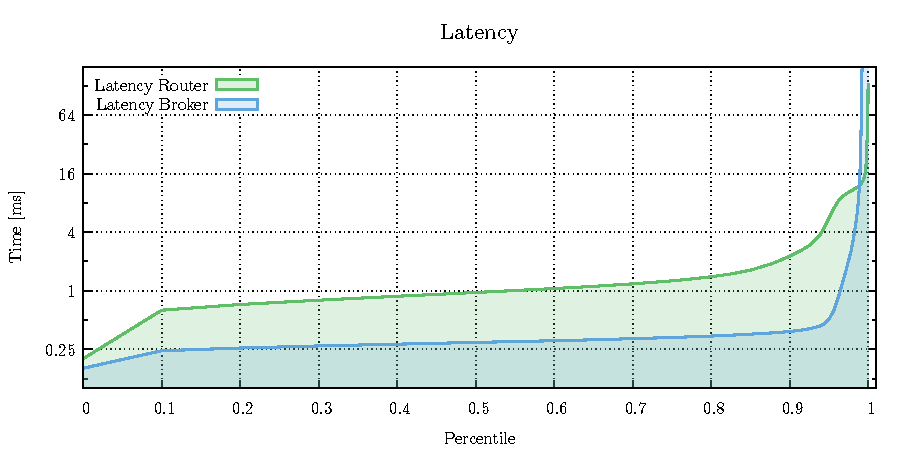
\includegraphics[width=1\linewidth]{obrazky-figures/charts/singlepoint-latency.pdf}
	\caption{Latency chart showing the difference between the router and the broker latency at 80\,\% of maximum rate. One can see that router is slower, but this is caused by the technology used in the Maestro Clients which is same as in the Broker..}
	\label{fig:latency-single-router}
\end{figure}

The memory used by Qpid-dispatch is slightly lower and much stable than in the case of maximum throughput as one can see in the Figure \ref{fig:latency-single-router-memory}. This proves, that used memory is mild to the  load. If the load on the router is higher than it needs more memory for proper routing. In the Figure \ref{fig:latency-single-broker-memory} one can see the Inspector output for Broker's used memory. The used memory is here much stable then in the previous cases, which is caused, as in the router case, by lower load on the Broker. Maximum used memory is same as in the previous cases.

\begin{figure}[H]
	\centering
	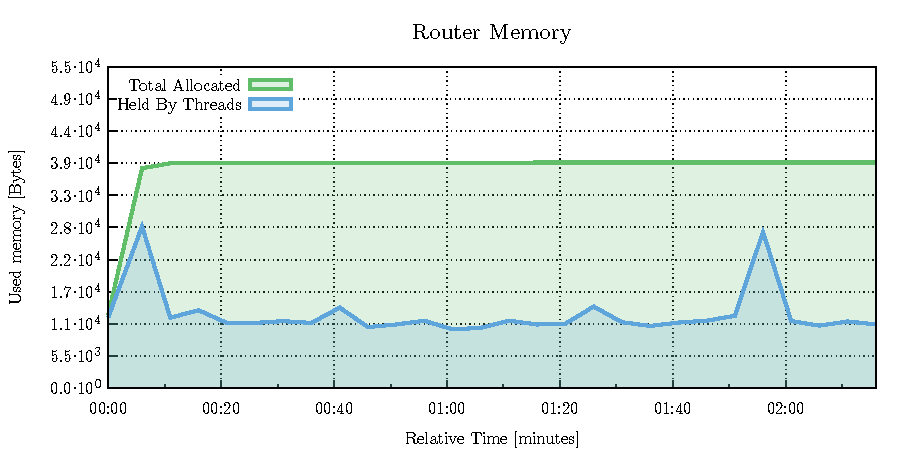
\includegraphics[width=1\linewidth]{obrazky-figures/charts/singlepoint-router-latency-memory.pdf}
	\caption{Memory usage of Qpid-Dispatch is much stable when the router is not under the maximum load. The spikes are caused by some unexpected events in the topology.}
	\label{fig:latency-single-router-memory}
\end{figure}

\begin{figure}[H]
	\centering
	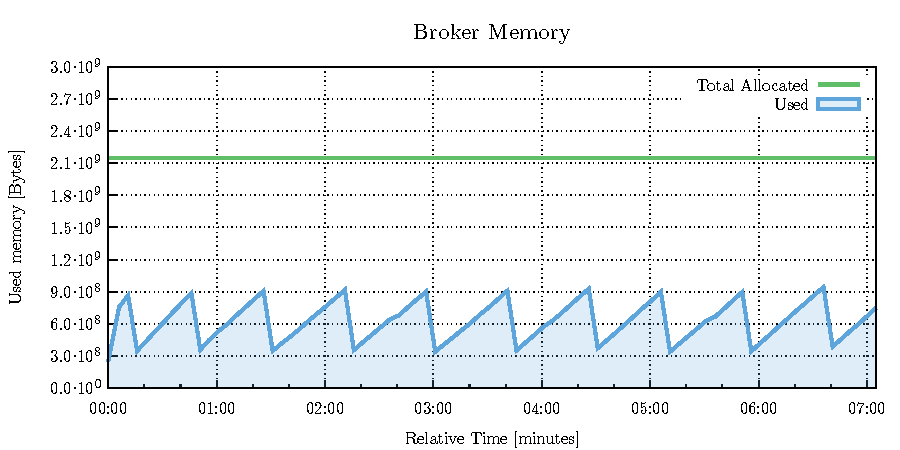
\includegraphics[width=1\linewidth]{obrazky-figures/charts/singlepoint-broker-latency-memory.pdf}
	\caption{The Broker's memory usage has lesser spike when the load is only about of 80\,\% of maximum.}
	\label{fig:latency-single-broker-memory}
\end{figure}

\subsubsection*{Multipoint Topology}
One can see the measured latency on multinode topology of three routers, and two routers with middle-broker in the Figure \ref{fig:latency-multipoint-router}. The latency curve proves, that routers are able to deliver messages into its destination faster than topology with the Broker, because the Broker needs to store them in the memory. The latency of the topology with broker reaches around 16\,$\mu$s in 90\,\% of samples; on the other hand, topology consisting of routers has significantly better latency that is around 1\,$\mu$s in 90\,\% of samples. The conclusion is that the collected data proves the router should be much faster than the broker during the certain circumstances..

\begin{figure}[H]
	\centering
	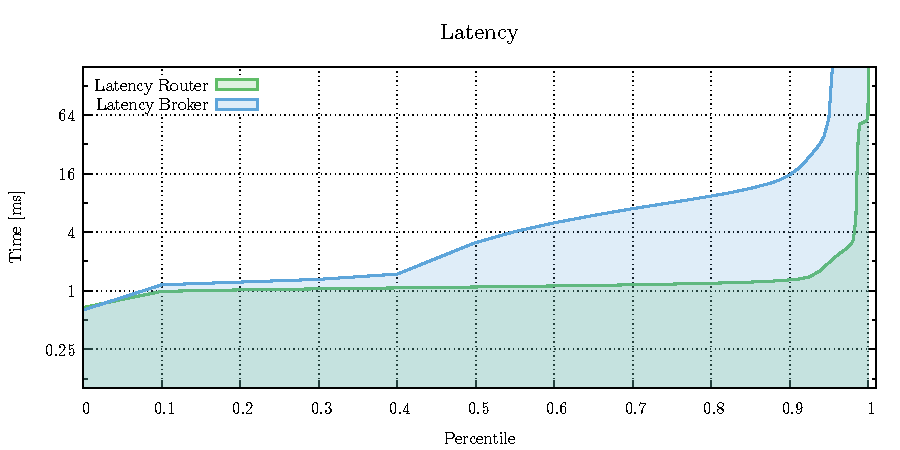
\includegraphics[width=1\linewidth]{obrazky-figures/charts/multipoint-latency.pdf}
	\caption{Latency comparison between topologies with only routers and with the middle-broker. The router network is here significantly faster.}
	\label{fig:latency-multipoint-router}
\end{figure}

\begin{figure}[H]
	\centering
	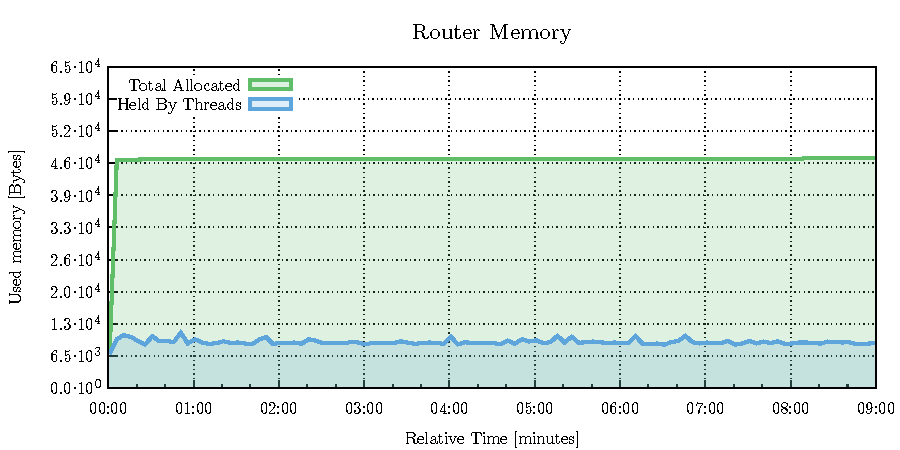
\includegraphics[width=1\linewidth]{obrazky-figures/charts/multipoint-router-only-latency-memory.pdf}
	\caption{Memory usage shows, that memory usage of the router is affected by the throughput.}
	\label{fig:latency-multiple-router-memory}
\end{figure}

Collected data about the memory usage proves the previous statements. In the Figure \ref{fig:latency-multiple-router-memory} is shown used memory by Qpid-Dispatch. The curve is very stable and the values moves around the 9\,MB of used memory. The used memory by the Broker shown in the Figure \ref{fig:latency-multiple-broker-memory} is very similar as in the previous measurements.

\begin{figure}[H]
	\centering
	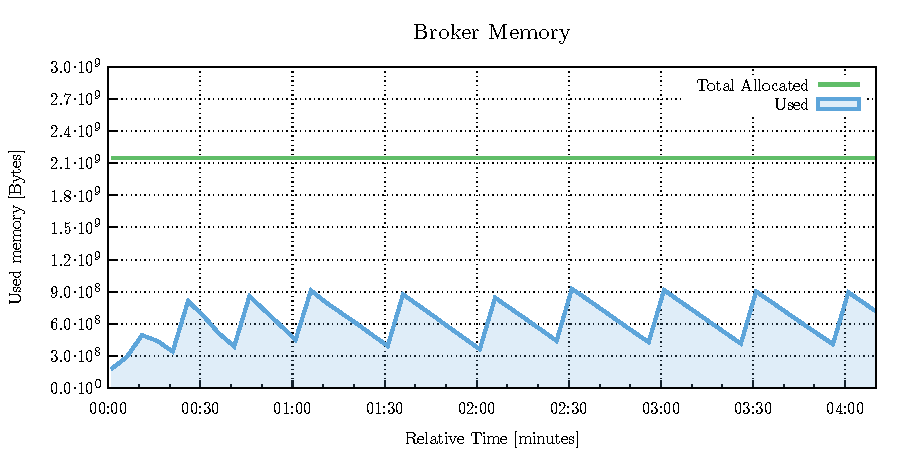
\includegraphics[width=1\linewidth]{obrazky-figures/charts/multipoint-router-broker-latency-memory.pdf}
	\caption{Chart of memory allocation on the Broker node..}
	\label{fig:latency-multiple-broker-memory}
\end{figure}

\subsubsection*{Conclusion}
During the latency measurements we collected and compared data for the Qpid-Dispatch and Message Broker topologies. The summary of latency measurements is available in the Table \ref{tab:latency-summary}. Is it was already mentioned, Qpid-Dispatch is faster in the model environment the Message Broker. How to achieve better comparison of latency measurements is discussed in the Section \ref{Maestro Clients in Python} as a part of possible improvements.

% Please add the following required packages to your document preamble:
% \usepackage{multirow}
% \usepackage[table,xcdraw]{xcolor}
% If you use beamer only pass "xcolor=table" option, i.e. \documentclass[xcolor=table]{beamer}
\begingroup
\setlength{\tabcolsep}{10pt} % Default value: 6pt
\renewcommand{\arraystretch}{1.35} % Default value: 1
	\begin{table}[H]
	\centering
	\caption{Table with collected latency data with highlighted performance improvements and degradations.}
	\label{tab:latency-summary}
	\begin{tabular}{|l|r|r|r|r|r|}
	\hline
	\rowcolor[HTML]{C5E3DF}
	\multicolumn{1}{|c|}{\cellcolor[HTML]{C5E3DF}}                                     & \multicolumn{2}{c|}{\cellcolor[HTML]{C5E3DF}\textbf{Latency (us)}}                                                        & \multicolumn{2}{c|}{\cellcolor[HTML]{C5E3DF}\textbf{Memory}}                                                                 & \multicolumn{1}{c|}{\cellcolor[HTML]{C5E3DF}}                                                                                         \\ \cline{2-5}
	\rowcolor[HTML]{C5E3DF}
	\multicolumn{1}{|c|}{\multirow{-2}{*}{\cellcolor[HTML]{C5E3DF}\textbf{Test Type}}} & \multicolumn{1}{c|}{\cellcolor[HTML]{C5E3DF}\textbf{90 \%}} & \multicolumn{1}{c|}{\cellcolor[HTML]{C5E3DF}\textbf{99 \%}} & \multicolumn{1}{c|}{\cellcolor[HTML]{C5E3DF}\textbf{Total}} & \multicolumn{1}{c|}{\cellcolor[HTML]{C5E3DF}\textbf{Used max}} & \multicolumn{1}{c|}{\multirow{-2}{*}{\cellcolor[HTML]{C5E3DF}\textbf{\begin{tabular}[c]{@{}c@{}}Duration \\ (seconds)\end{tabular}}}} \\ \hline
	\textbf{Single Router}                                                             & 2.263                                                       & 12.495                                                      & 38 KB                                                       & 28 KB                                                          & \cellcolor[HTML]{9AFF99}136                                                                                                           \\ \hline
	\textbf{Single Broker}                                                             & 0.386                                                       & 181.759                                                     & 2 GB                                                        & 0.9 GB                                                         & \cellcolor[HTML]{FFCCC9}425                                                                                                           \\ \hline
	\textbf{Line of Routers}                                                           & \cellcolor[HTML]{9AFF99}1.292                               & 50.815                                                      & 46 KB                                                       & 8 KB                                                           & \cellcolor[HTML]{FFCCC9}540                                                                                                           \\ \hline
	\textbf{Line with Broker}                                                          & \cellcolor[HTML]{FFCCC9}15.487                              & 1031.167                                                    & 2 GB                                                        & 0.9 GB                                                         & \cellcolor[HTML]{9AFF99}250                                                                                                           \\ \hline
	\end{tabular}
	\end{table}
\endgroup

\newpage
\section{Behavior Measurements}
\label{Behavior Measurements}

\todo{Tohle popsat az s~nejakym dalsim merenim, zatim asi netreba kontrlovat, pouze prevzato z~Excelu}

\subsection{Agent Evaluation}
Moreover, we present some preliminary results with using the agent extension and changing the behavior of topology depicted in the Figure \ref{fig:basic_topologies}. In the Figure \ref{fig:agent_throughput} you can see throughput of few simple tests during which middle router is restarted or shut down. The throughput spikes are caused by these events. Since router does not have any queues to store messages, the messages are then discarded and lost. However, the sender does not receive acknowledgment of lost messages so it is not router responsibility. In the Table \ref{tab:agent_simple} you can see the duration of each executed operation and rate of lost messages during the operation (with expected amount of messages being 10\,000\,000). For example during the restart, router was completely shutdown for a second during which no messages arrived. However, after the restart there was some time to balance the load to the previous point. This leads to message lost equals to 2 seconds rate.

% Please add the following required packages to your document preamble:
% \usepackage[table,xcdraw]{xcolor}
% If you use beamer only pass "xcolor=table" option, i.e. \documentclass[xcolor=table]{beamer}
\begin{table}[H]
\centering
\caption{Summarization of lost messages during the connection issues.}
\label{my-label}
\begin{tabular}{|c|r|r|}
\hline
\rowcolor[HTML]{C5E3DF}
Operation     & Duration (seconds) & Message Lost \\ \hline
None          & 0        & None         \\ \hline
Restart       & 1        & 46437        \\ \hline
Shutdown      & 12       & 280572       \\ \hline
Long Shutdown & 89       & 1304451      \\ \hline
\end{tabular}
\label{tab:agent_simple}
\end{table}

The Figure \ref{fig:agent_throughput} also shows, that test case with long shutdown is longer about 10 seconds that other scenarios and the throughput after the shutdown is quite higher. This means that router high throughput to even the messages lost.

\begin{figure}[H]
	\centering
	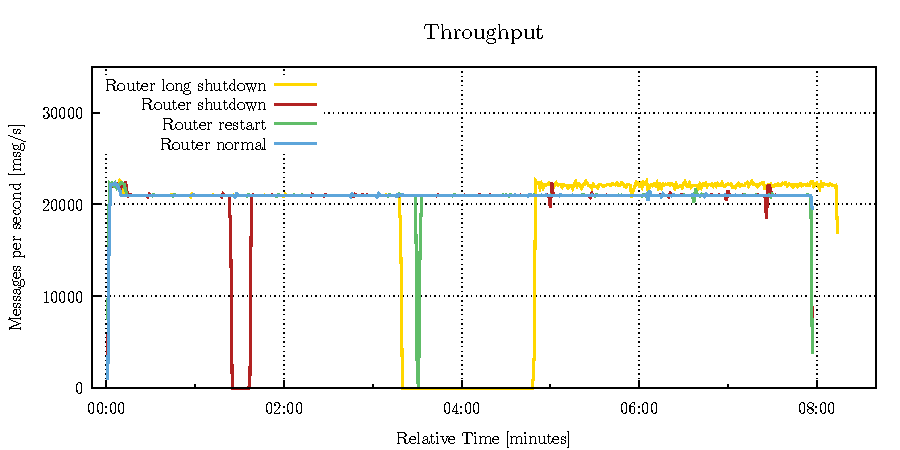
\includegraphics[width=1\linewidth]{obrazky-figures/charts-excel/agent.pdf}
	\caption{Router throughput comparison during the same load after different unexpected events.}
	\label{fig:agent_throughput}
\end{figure}

Latency of test cases cases with the agent function demonstration is depicted in the Figure \ref{fig:agent_latency}. You can see that router is able to even the latency during the restart and short shutdown with test run without any unexpected behavior. On the other hand, long shutdown (red) gets worse latency almost for 50 percentile of messages.

\begin{figure}[H]
	\centering
	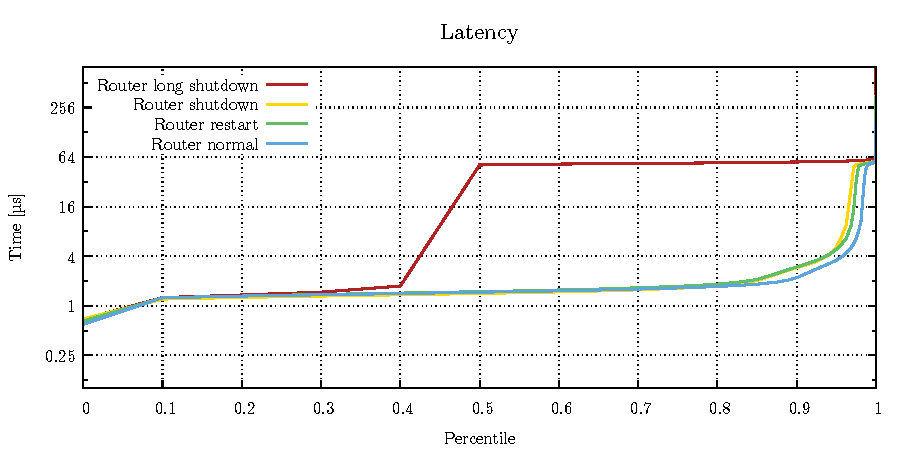
\includegraphics[width=1\linewidth]{obrazky-figures/charts-excel/agent_latency.pdf}
	\caption{Router and broker latency comparison during the same load.}
	\label{fig:agent_latency}
\end{figure}


\section{Problems}

All measurements were orchestrated by an automation server called Jenkins\footnote{Jenkins\,---\,\url{https://jenkins.io/}}.
